\documentclass[border=5mm,tikz]{standalone} 

\usepackage{amsmath}
% !TEX root=img/arguments_and_attack.tex

% \usetikzlibrary{external} 
% \tikzexternalize[prefix=tikz/] 

\usetikzlibrary{calc}
\usetikzlibrary{arrows}
\usetikzlibrary{arrows.meta}
\usetikzlibrary{decorations.markings}
% \usetikzlibrary{intersections}
\usetikzlibrary{fit}
\usetikzlibrary{shapes}
% \usetikzlibrary{trees}


\tikzset{
	every path/.style={thick},
	align=center,
	observed/.style={
		fill=black!20,
	},
	bn/.style={
		draw,
		ellipse,
		-{Triangle[angle=60:6pt 0]}
	},
	scn/.style={
		draw,
		rectangle,
		% signal,
		% signal from=west,
		% signal pointer angle=120,
		-{Triangle[angle=60:6pt 0]},
	},
	possibly/.style={dashed},
	arg/.style={
		draw,
		rectangle,
		-{Straight Barb[angle=60:6pt 0]}
	},
	attack/.style={
		-{Rays[width=10pt,length=10pt,sep=-3.9pt]}
	},
	pref/.style={
		draw,
		rectangle,
		-{Straight Barb[angle=60:6pt 0]}
	},
	subscn/.style={
		double,
		-{Triangle[angle=60:6pt 0]},
	},
	specific/.style={
		double,
		-{Stealth[angle=60:6pt 0]}
	},
}



\begin{document}
	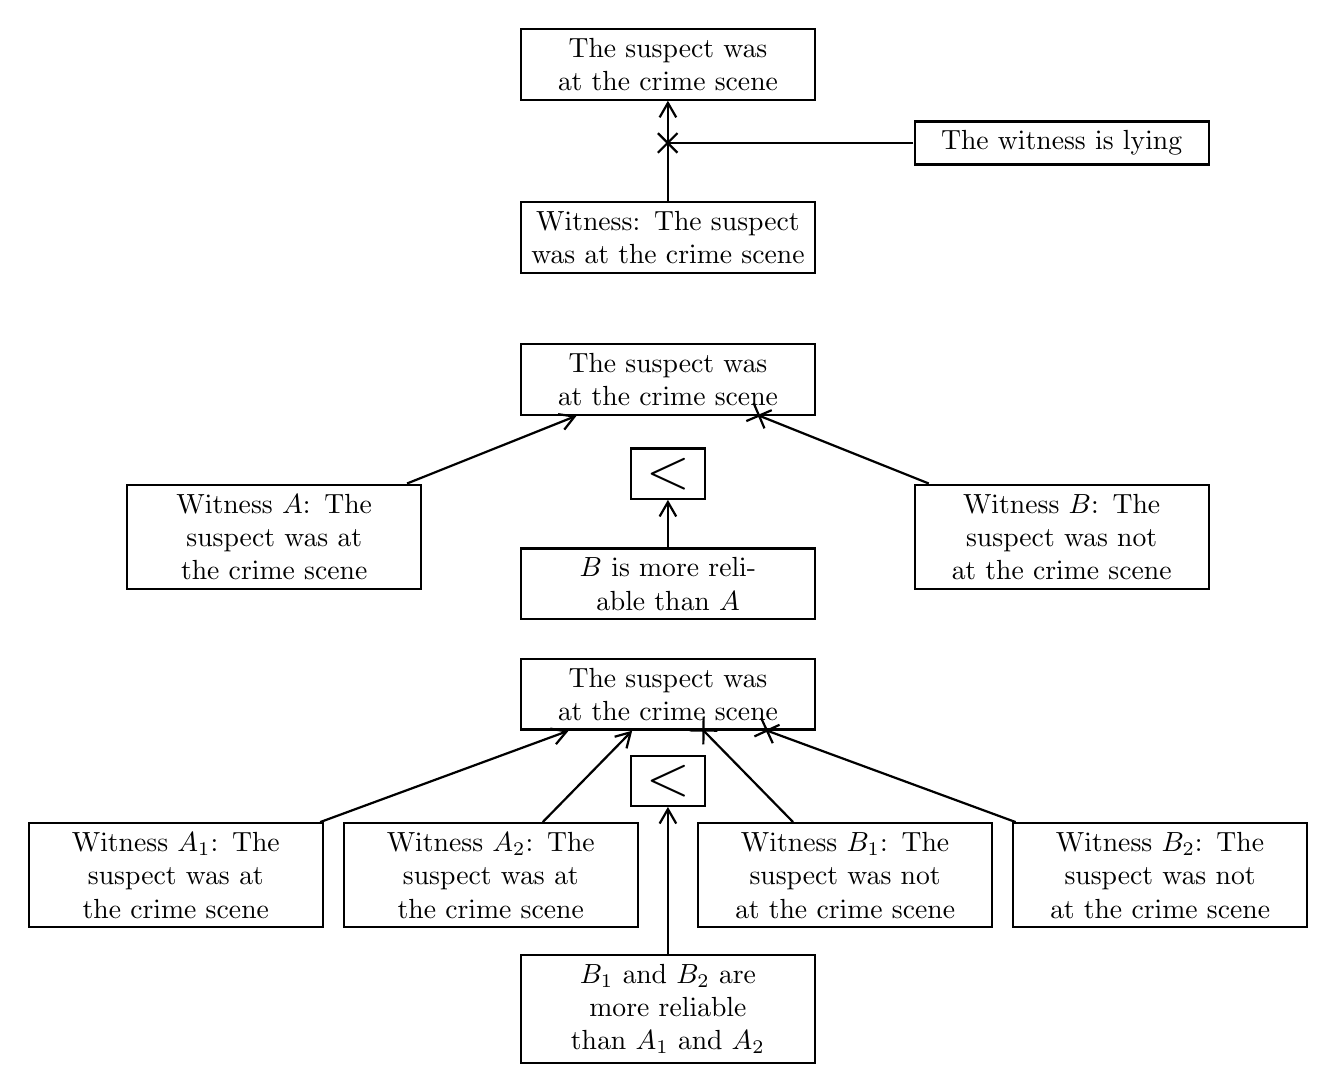
\begin{tikzpicture}[
		scnnode/.append style={text width=3cm},
		arg/.append style={text width=3.5cm},
		pref/.append style={text width=0.7cm},
	]
		\pgftransformxscale{5}
		\pgftransformyscale{2}


		\node[arg]     			(scene) at (0,0) {The suspect was at the crime scene};
		\node[arg] (witn) at (0,-1.1) {Witness: The suspect was at the crime scene};

		\node[arg] 					(lying) at (1,-0.5) {The witness is lying};

		\draw[arg] 					(witn) -- (scene);
		\draw[attack] 			(lying) -- (0, -0.5);

%*********

		\node[arg]     			(scene) at (0,-2) {The suspect was at the crime scene};
		\node[arg] (witn) at (-1,-3) {Witness $A$: The suspect was at the crime scene};
		\node[arg] (witn2) at (1,-3) {Witness $B$: The suspect was not at the crime scene};

		\draw[arg] 					(witn) -- (scene);
		\draw[attack] 			(witn2) -- (scene);

		\node[pref] 				(pref) at (0,-2.6) 	{\huge $<$};
		\node[arg] 					(rel) at (0,-3.3) 		{$B$ is more reliable than $A$};

		\draw[arg] 					(rel) -- (pref);

%*********

		\node[arg]     			(scene) at (0,-4) {The suspect was at the crime scene};
		\node[arg] (witn) at (-1.25,-5.15) {Witness $A_1$: The suspect was at the crime scene};
		\node[arg] (witn2) at (-0.45,-5.15) {Witness $A_2$: The suspect was at the crime scene};
		\node[arg] (witn3) at (0.45,-5.15) {Witness $B_1$: The suspect was not at the crime scene};
		\node[arg] (witn4) at (1.25,-5.15) {Witness $B_2$: The suspect was not at the crime scene};

		\draw[arg] 					(witn) -- (scene);
		\draw[arg] 					(witn2) -- (scene);
		\draw[attack] 			(witn3) -- (scene);
		\draw[attack] 			(witn4) -- (scene);

		\node[pref] 				(pref2) at (0,-4.55) 	{\huge $<$};
		\node[arg] 					(outweigh) at (0,-6) 		{$B_1$ and $B_2$ are more reliable than $A_1$ and $A_2$};

		\draw[arg] 					(outweigh) -- (pref2);



	\end{tikzpicture}
\end{document}
